
\nonstopmode
\documentclass{standalone}

% This document contains the TikZ-header for all our LaTeX-computations.
% It especially contains all global graphic parameters.

\usepackage{amsmath, amssymb, amsfonts} % Standard Math-stuff

\usepackage{tikz}
\usetikzlibrary{calc}
\usetikzlibrary{positioning}

% Define a text=none option for nodes that ignores the given text, from
% https://tex.stackexchange.com/questions/59354/no-text-none-in-tikz
\makeatletter
\newif\iftikz@node@phantom
\tikzset{
  phantom/.is if=tikz@node@phantom,
  text/.code=%
    \edef\tikz@temp{#1}%
    \ifx\tikz@temp\tikz@nonetext
      \tikz@node@phantomtrue
    \else
      \tikz@node@phantomfalse
      \let\tikz@textcolor\tikz@temp
    \fi
}
\usepackage{etoolbox}
\patchcmd\tikz@fig@continue{\tikz@node@transformations}{%
  \iftikz@node@phantom
    \setbox\pgfnodeparttextbox\hbox{}
  \fi\tikz@node@transformations}{}{}
\makeatother

% Now we define the global styles
% The global styles are defined nestedly. You have to give your tikzpicture
% the global options [vertexStyle, edgeStyle, faceStyle] to activate them.
% 
% You can disable labels by using the option nolabels, i.e. 
% vertexStyle=nolabels to deactivate vertex labels.
%
% If you want to have a specific style for your picture, you can also use
% this specific meta-style instead of the general style. For example if you
% want to use double edges in one single picture - no matter the style of
% the rest of the document - you can use edgeDouble instead of edgeStyle.
%
% To set the default style, modify the vertexStyle/.default entry.

% Vertex styles
\tikzset{ 
    vertexNodePlain/.style = {fill=gray, shape=circle, inner sep=0pt, minimum size=2pt, text=none},
    vertexPlain/labels/.style = {
        vertexNode/.style={vertexNodePlain},
        vertexLabel/.style={gray}
    },
    vertexPlain/nolabels/.style = {
        vertexNode/.style={vertexNodePlain},
        vertexLabel/.style={text=none}
    },
    vertexPlain/.style = vertexPlain/#1,
    vertexPlain/.default=labels
}
\tikzset{
    vertexNodeNormal/.style = {fill=blue, shape=circle, inner sep=0pt, minimum size=4pt, text=none},
    vertexNormal/labels/.style = {
        vertexNode/.style={vertexNodeNormal},
        vertexLabel/.style={blue}
    },
    vertexNormal/nolabels/.style = {
        vertexNode/.style={vertexNodeNormal},
        vertexLabel/.style={text=none}
    },
    vertexNormal/.style = vertexNormal/#1,
    vertexNormal/.default=labels
}
\tikzset{
    vertexNodeBall/.style = {shape=circle, ball color=orange, inner sep=2pt, outer sep=0pt, minimum size=3pt},
    vertexBall/labels/.style = {
        vertexNode/.style={vertexNodeBall, text=black},
        vertexLabel/.style={text=none}
    },
    vertexBall/nolabels/.style = {
        vertexNode/.style={vertexNodeBall, text=none},
        vertexLabel/.style={text=none}
    },
    vertexBall/.style = vertexBall/#1,
    vertexBall/.default=labels
}
\tikzset{ 
    vertexStyle/.style={vertexNormal=#1},
    vertexStyle/.default = labels
}


% 1) position of the vertex
% 2) relative position of the node
% 3) name of the vertex
\newcommand{\vertexLabelR}[3]{
    \node[vertexLabel, #2] at (#1) {#3};
}
% 1) position of the vertex
% 2) absolute position of the node
% 3) name of the vertex
\newcommand{\vertexLabelA}[3]{
    \node[vertexLabel] at (#2) {#3};
}


% Edge styles
% If you have trouble with the double-lines overlapping, this might (?) help:
% https://tex.stackexchange.com/questions/288159/closing-the-ends-of-double-line-in-tikz
\tikzset{
    edgeLinePlain/.style={line join=round},
    edgePlain/labels/.style = {
        edge/.style={edgeLinePlain},
        edgeLabel/.style={fill=blue!20!white}
    },
    edgePlain/nolabels/.style = {
        edge/.style={edgeLinePlain},
        edgeLabel/.style={text=none}
    },
    edgePlain/.style = edgePlain/#1,
    edgePlain/.default = labels
}
\tikzset{
    edgeLineDouble/.style = {thin, double=gray!90!white, double distance=.3pt, line join=round},
    edgeDouble/labels/.style = {
        edge/.style = {edgeLineDouble},
        edgeLabel/.style = {fill=blue!20!white}
    },
    edgeDouble/nolabels/.style = {
        edge/.style = {edgeLineDouble},
        edgeLabel/.style = {text=none}
    },
    edgeDouble/.style = edgeDouble/#1,
    edgeDouble/.default = labels
}
\tikzset{
    edgeStyle/.style = {edgePlain=#1},
    edgeStyle/.default = labels
}

% Face styles
% Here we have an exception - the style face is always defined.
% 
\newcommand{\faceColorY}{yellow!60!white}   % yellow
\newcommand{\faceColorB}{blue!60!white}     % blue
\newcommand{\faceColorP}{cyan!60}           % purple
\newcommand{\faceColorR}{red!60!white}      % red
\newcommand{\faceColorG}{green!60!white}    % green
\newcommand{\faceColorO}{orange!50!yellow!70!white} % orange

\newcommand{\faceColor}{\faceColorY}
\newcommand{\faceColorSwap}{\faceColorB}
\tikzset{
    face/.style = {fill=#1},
    face/.default = \faceColor,
    faceY/.style = {face=\faceColorY},
    faceB/.style = {face=\faceColorB},
    faceP/.style = {face=\faceColorP},
    faceR/.style = {face=\faceColorR},
    faceG/.style = {face=\faceColorG},
    faceO/.style = {face=\faceColorO}
}
\tikzset{
    faceStyle/labels/.style = {
        faceNode/.style = {}
    },
    faceStyle/nolabels/.style = {
        faceNode/.style = {text=none}
    },
    faceStyle/.style = faceStyle/#1,
    faceStyle/.default = labels
}
\tikzset{ face/.style={fill=#1} }
\tikzset{ faceSwap/.code=
    \ifdefined\swapColours
        {face=\faceColorSwap}
    \else
        {face=\faceColor}
    \fi
}

% Sometimes we want to implement different behaviour for the generated 
% HTML-pictures (for example, shading is not supported in HTML).
% For that we define a macro to check whether we run the code with
% htlatex. The code comes from 
% https://tex.stackexchange.com/questions/93852/what-is-the-correct-way-to-check-for-latex-pdflatex-and-html-in-the-same-latex
\makeatletter
\edef\texforht{TT\noexpand\fi
  \@ifpackageloaded{tex4ht}
    {\noexpand\iftrue}
    {\noexpand\iffalse}}
\makeatother


\usepackage{hyperref}


\def\pgfsysdriver{pgfsys-tex4ht.def}

\begin{document}
       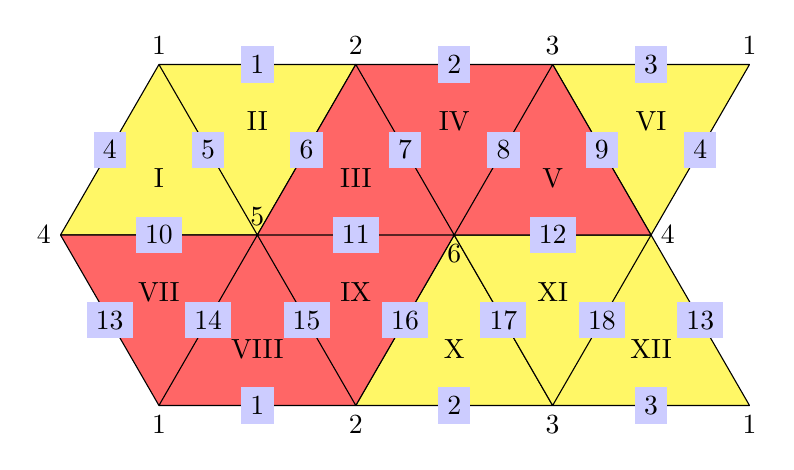
\begin{tikzpicture}[vertexStyle=nolabels,edgePlain,faceStyle]
         \def\edgeFacePath{1}
         \def\dist{2.5}

\coordinate (A1) at (0,0);
\coordinate (B1) at (\dist,0);
\coordinate (C1) at ($2*(B1)$);
\coordinate (A2) at ($3*(B1)$);
\coordinate (D1) at (120:\dist);
\coordinate (E) at ($(B1)+(D1)$);
\coordinate (F) at ($(B1)+(E)$);
\coordinate (D2) at ($(C1)+(E)$);
\coordinate (A3) at ($(D1)+(E)$);
\coordinate (B2) at ($2*(E)$);
\coordinate (C2) at ($(B1)+(B2)$);
\coordinate (A4) at ($(B2)+(C1)$);

\tikzset{customFace/.style={face=\faceColorR}}
\draw[face,edge]
    (D1) -- (E) -- (A3) -- node[edgeLabel]{4} cycle
    (A3) -- node[edgeLabel]{5} (E) -- (B2) -- node[edgeLabel]{1} cycle
    (C2) -- (D2) -- node[edgeLabel]{4} (A4) -- node[edgeLabel]{3} cycle
    (B1) -- node[edgeLabel]{2} (C1) -- (F) -- cycle;
\draw[edge,\ifdefined\longEdgeFacePath customFace\else face\fi]
    (C1) -- node[edgeLabel]{17} (F) -- (D2) -- cycle
    (C1) -- node[edgeLabel]{18} (D2) -- node[edgeLabel]{13} (A2) -- node[edgeLabel]{3} cycle;
\draw[edge,\ifdefined\edgeFacePath customFace\else face\fi]
    (E) -- node[edgeLabel]{6} (B2) -- (F) -- cycle
    (B2) -- node[edgeLabel]{7} (F) -- (C2) -- node[edgeLabel]{2} cycle
    (F) -- node[edgeLabel]{8} (C2) -- node[edgeLabel]{9} (D2) -- node[edgeLabel]{12} cycle
    (A1) -- node[edgeLabel]{13} (D1) -- node[edgeLabel]{10} (E) -- cycle
    (A1) -- node[edgeLabel]{1} (B1) -- (E) -- node[edgeLabel]{14} cycle
    (B1) -- node[edgeLabel]{15} (E) -- node[edgeLabel]{11} (F) -- node[edgeLabel]{16} cycle;


\foreach \a/\b/\c/\n in {A3/E/D1/I, A3/B2/E/II, B2/F/E/III, B2/C2/F/IV, C2/D2/F/V, C2/A4/D2/VI, D1/E/A1/VII, E/B1/A1/VIII, E/F/B1/IX, F/C1/B1/X, F/D2/C1/XI, D2/A2/C1/XII}{
    \node at (barycentric cs:\a=1,\b=1,\c=1) {\n};
}

\foreach \p/\r/\n in {A3/above/1, B2/above/2, C2/above/3, A4/above/1, D1/left/4, E/above/5, F/below/6, D2/right/4, A1/below/1, B1/below/2, C1/below/3, A2/below/1}{
    \vertexLabelR{\p}{\r}{\n}
}


       \end{tikzpicture}
     </Alt>

     @InsertChunk Definition_EdgeFacePath

     @ExampleSession
 gap> edgeFacePath := EdgeFacePath( thinTorus, [13,7,14,8,15,9,11,3,7,4,8,5,9] );
 | e13, F7, e14, F8, e15, F9, e11, F3, e7, F4, e8, F5, e9 |
 gap> IsEdgeFacePath(edgeFacePath);
 true
 gap> IsList(edgeFacePath);
 false
 gap> IsEdgeFacePath( [13,7,14,8,15,9,11,3,7,4,8,5,9] );
 false
     @EndExampleSession
  
     The elements of a vertex-edge-path can be accessed by using the methods
     <K>PathAsList</K> (<Ref Subsect="EdgeFace_PathAsList"/>),
     <K>EdgesAsList</K> (<Ref Subsect="EdgeFace_EdgesAsList"/>) and 
     <K>FacesAsList</K> (<Ref Subsect="EdgeFace_FacesAsList"/>).

     The NC-version does not check if the
     given <A>path</A> is a list 
     <M>[e_1,f_1,e_2,f_2,\ldots,e_n,f_n,e_{{n+1}}]</M> that fulfills these
     conditions.
   </Description>
 </ManSection>
No AutoDoc-documentation since the order of the next two entries should
be switched
clareOperation( "EdgeFacePath", [IsPolygonalComplex, IsDenseList] );
clareOperation( "EdgeFacePathNC", [IsPolygonalComplex, IsDenseList] );

 @BeginGroup EdgeFacePathByEdges
 @Description
 Construct a new edge-face-path (<Ref Subsect="EdgeFacePath"/>) from a
 polygonal complex and a dense list of edges. Every two adjacent edges
 have to be connected by a face. If there are multiple such faces, the one
 with the smallest label is used. If the given <A>edgeList</A> is empty,
 <K>fail</K> is returned.

 With this the paths from <Ref Subsect="EdgeFacePath"/> can be defined
 more compactly:
 @BeginExampleSession
 gap> edgeFacePath:=EdgeFacePathByEdges(thinTorus,[13,14,15,11,7,8,9]);
 | e13, F7, e14, F8, e15, F9, e11, F3, e7, F4, e8, F5, e9 |
 gap> IsEdgeFacePath(edgeFacePath);
 true
 @EndExampleSession

 The NC-version does not check whether the given <A>edgeList</A> consists
 of edges in <A>complex</A> and whether every two adjacent edges are
 connected by an face.

 @Returns a edge-face-path or <K>fail</K>
 @Arguments complex, vertexList
clareOperation( "EdgeFacePathByEdges", [IsPolygonalComplex, IsDenseList] );
 @Arguments complex, edgeList
clareOperation( "EdgeFacePathByEdgesNC", [IsPolygonalComplex, IsDenseList] );
 @EndGroup


 @BeginGroup EdgeFacePathByFaces
 @Description
 Construct a new edge-face-path (<Ref Subsect="EdgeFacePath"/>) from a
 polygonal complex and a dense list of faces. Every two adjacent faces
 have to be connected by an edge.
 The first and the last edge are not clearly given by the faces. 
 So by default they are an edge which is not between the first and the 
 second face and not between the penultimate and the last edge. 
 If different edges are available inner edges are preferred and the 
 smallest possible edge is chosen.

 With this the paths from <Ref Subsect="EdgeFacePath"/> can be defined
 more compactly:
 @BeginExampleSession
 gap> edgeFacePath1:=EdgeFacePathByFaces(thinTorus,[7,8,9,3,4,5],10,9);
 | e10, F7, e14, F8, e15, F9, e11, F3, e7, F4, e8, F5, e9 |
 gap> IsEdgeFacePath(edgeFacePath1);
 true
 gap> edgeFacePath2:=EdgeFacePathByFaces(thinTorus,[7,8,9,3,4,5]);
 | e10, F7, e14, F8, e15, F9, e11, F3, e7, F4, e8, F5, e9 |
 gap> IsEdgeFacePath(edgeFacePath2);
 true
 @EndExampleSession
 Also for faces with the same edges you can build the edge-face-path by faces:
 @BeginExampleSession
 gap> EdgeFacePathByFaces(JanusHead(),[1,2]);
 ( e1, F1, e2, F2, e1 )
 @EndExampleSession 

 The NC-version does not check whether the given <A>faceList</A> consists
 of faces in <A>complex</A>.

 @Returns a edge-face-path
 @Arguments complex, faceList[, firstEdge, lastEdge]
clareOperation( "EdgeFacePathByFaces", [IsPolygonalComplex, IsDenseList, IsPosInt, IsPosInt] );
 @Arguments complex, faceList[, firstEdge, lastEdge]
clareOperation( "EdgeFacePathByFacesNC", [IsPolygonalComplex, IsDenseList, IsPosInt, IsPosInt] );
 @EndGroup

 @BeginGroup EdgeFace_PathAsList
 @Description
   Return the complete edge-face-path as a list (with edges and
   faces alternating), starting with an edge.
   
   For the examples from <K>EdgeFacePath</K> 
   (<Ref Subsect="EdgeFacePath"/>) in the simplicial surface from the 
   start of section <Ref Sect="Section_Paths_EdgeFace"/>:
   @ExampleSession
 gap> edgeFacePath;
 | e13, F7, e14, F8, e15, F9, e11, F3, e7, F4, e8, F5, e9 |
 gap> PathAsList( edgeFacePath );
 [ 13, 7, 14, 8, 15, 9, 11, 3, 7, 4, 8, 5, 9 ]
   @EndExampleSession
 @Arguments edgeFacePath
 @Returns a list of positive integers
clareAttribute( "PathAsList", IsEdgeFacePath );
 @EndGroup

 @BeginGroup EdgeFace_EdgesAsList
 @Description
   Return the edges of the edge-face-path as a list.

   For the examples from <K>EdgeFacePath</K> 
   (<Ref Subsect="EdgeFacePath"/>) in the simplicial surface from the 
   start of section <Ref Sect="Section_Paths_EdgeFace"/>:
   @ExampleSession
 gap> edgeFacePath;
 | e13, F7, e14, F8, e15, F9, e11, F3, e7, F4, e8, F5, e9 |
 gap> EdgesAsList( edgeFacePath );
 [ 13, 14, 15, 11, 7, 8, 9 ]
   @EndExampleSession
 @Arguments edgeFacePath
 @Returns a list of positive integers
clareAttribute( "EdgesAsList", IsEdgeFacePath );
 @EndGroup

 @BeginGroup EdgeFace_FacesAsList
 @Description
     Return the faces of the edge-face-path as a list.

   For the examples from <K>EdgeFacePath</K> 
   (<Ref Subsect="EdgeFacePath"/>) in the simplicial surface from the 
   start of section <Ref Sect="Section_Paths_EdgeFace"/>:
   @ExampleSession
 gap> edgeFacePath;
 | e13, F7, e14, F8, e15, F9, e11, F3, e7, F4, e8, F5, e9 |
 gap> FacesAsList( edgeFacePath );
 [ 7, 8, 9, 3, 4, 5 ]
   @EndExampleSession
 @Arguments edgeFacePath
 @Returns a list of positive integers
clareAttribute( "FacesAsList", IsEdgeFacePath );
 @EndGroup


 <ManSection Label="EdgeFace_IsClosedPath">
   <Prop Name="IsClosedPath" Arg="edgeFacePath"
     Label="for IsEdgeFacePath"
     Comm="Return whether the given path is closed"/>
   <Returns><K>true</K> or <K>false</K></Returns>
   <Description>
     Check whether the given edge-face-path is closed, i.e. whether
     the first and last vertex in this path are equal.

 The example from <K>EdgeFacePath</K>
 (<Ref Subsect="EdgeFacePath"/>) is not closed but an extended version
 of the path is.
  <Alt Only="HTML">
 &lt;br>&lt;img src="./images/_Wrapper_Image_ThinTorus_longPath-1.svg"> &lt;/img> &lt;br>
end{document}